
%(BEGIN_QUESTION)
% Copyright 2012, Tony R. Kuphaldt, released under the Creative Commons Attribution License (v 1.0)
% This means you may do almost anything with this work of mine, so long as you give me proper credit

The {\it Pythagorean Theorem} is a mathematical relationship between the lengths of the sides of a right triangle.  Sometimes this relationship is represented graphically:

$$
\includegraphics[width=15.5cm]{i02676x01.eps}$$

Explain how this geometrical illustration relates to the Pythagorean Theorem ($c^2 = a^2 + b^2$).

\underbar{file i02676}
%(END_QUESTION)





%(BEGIN_ANSWER)

This illustration represents the Pythagorean Theorem in geometric form: the {\it squares} of the lengths of the opposite and adjacent sides, when added, equal the {\it square} of the length of the hypotenuse.

$$\includegraphics[width=15.5cm]{i02676x02.eps}$$

The side lengths of this triangle are 6, 8, and 10.  Their corresponding areas are 36, 64, and 100.

%(END_ANSWER)





%(BEGIN_NOTES)


%INDEX% Mathematics review: trigonometric calculations

%(END_NOTES)


